\documentclass[UTF8]{article}

%--
\usepackage{ctex}
\usepackage[margin=1in]{geometry}
\usepackage{graphicx}
\usepackage{subfigure}
\usepackage{multirow}
\usepackage{algorithm}
\usepackage{algpseudocode}
\usepackage{amsmath}
%\usepackage[top=2cm, bottom=2cm, left=2cm, right=2cm]{geometry}
\usepackage{algorithmicx}
\usepackage{algpseudocode}


%\floatname{algorithm}{算法}
\renewcommand{\algorithmicrequire}{\textbf{Input:}}
\renewcommand{\algorithmicensure}{\textbf{Output:}}

%--
\begin{document}
    
%--
{\flushleft \bf \Large 主题:} 分布式系统大作业-Raft实验报告

{\flushleft \bf \Large 姓名:} 黄彬寓

{\flushleft \bf \Large 学号:} MF20330030

{\flushleft \bf \Large 日期:} 2020.12.28

\section{分析与设计}

\subsection{step1.设计Raft及四类RPC结构体}
首先是最重要的Raft结构体,除了原有的锁、集群内的serverID、自己的ID等数据外,根据Raft论文的Figure2,我们可以把所有servers的持久化数据(currentTerm、voteFor、log数组)、易挥发数据( commitIndex、lastApplied)、leader专属数据(nextIndex数组、matchIndex数组)都写入结构体中,再加上自己定义的为了更方便处理的变量和heartbeat、election定时器以及模拟状态机的ApplyMsg类型的信道。其中日志log是需要我们自己定义的,根据论文题意,显然放入Index、term、command这三项数据是合理且足够的。

接着定义RequestVoteArgs、RequestVoteReply、AppendEntriesArgs、AppendEntriesReply这四个结构体,其中前三个结构体按照Fugure2实现已经能够满足需要,而AppendEntriesReply中,为了能够让nextIndex快速回退或快速推进,需要额外定义一些变量。

\subsection{step2.设计Make与Start,完成总体框架}
首先,我先完善Make()与Start()这两个函数,因为这两个函数是通过外部接口调用的,Make()实现一个server节点的各种任务,Start()实现client向server发送request。

在Make()中,首先完成对rf结构体的初始化,如果之前保存了持久化数据,则调用readPersist读取;随后是一个大的循环,在该循环内,除非触发了Kill(),否则认为该server没有奔溃,持续运行,该循环体我定义为Loop()函数。设计Loop()的思路是这样的,除了client发出request、收到RequestVote和 AppendEntries RPC外,所有可能的操作都会在Loop()(或被Loop()调用的函数)中发生。那么显然,我们按照server的角色或者定时器到点这两种逻辑来设计Loop()是更合理的。这里Loop()的伪代码在图1中显示,我使用的是外层循环为定时器,内层循环为rf的角色状态。

\begin{figure}[h]
  \centering
  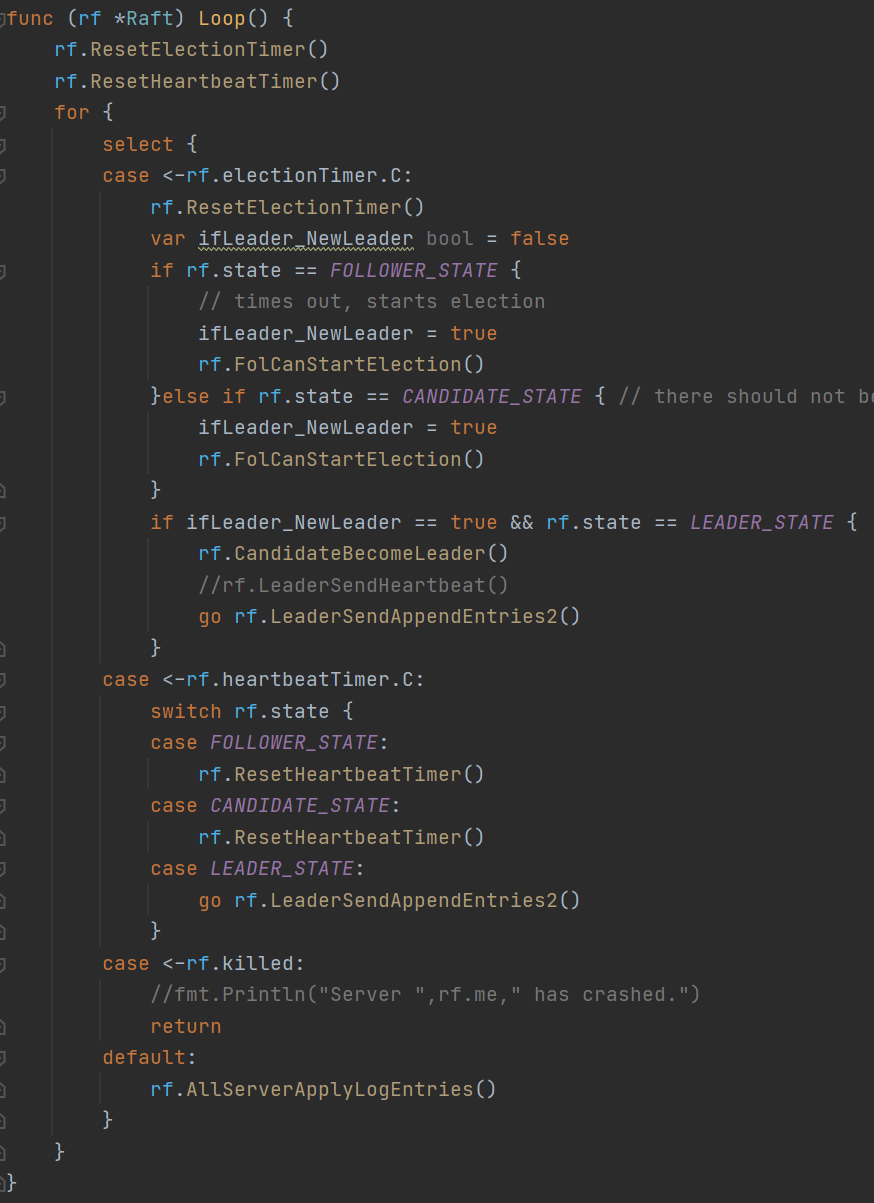
\includegraphics[scale=0.3]{pic1.png}
  \caption{框架函数Loop}
 %% \Description{This is an example of list in distributed systems.}
\end{figure}

在election定时器到时,根据当前状态,若为follower或candidate则开始进行选举,若为leader则跳过,但是考虑到这也可以是选举完刚产生的leader,所以使用一个bool变量来判断是否是新当前新选举出的leader,若是则立刻执行发送heartbeat通报给其他servers。

在heartbeat定时器到时,根据当前状态,若为follower或candidate则重置定时器并跳出,若为leader则发送heartbeat并在内部重置heartbeat定时器。这里我为了加快日志复制的效率,将系统中所有的heartbeat也当作普通的AppendEntries来发送,区别仅在于这样使普通的heartbeat也能够附带上日志,加快复制进度。

在Start函数中,我们需要做的是模拟server收到来自某一个client发出的request。那么首先判断该server是否是leader,如果不是应该将该request转交给leader或者拒绝该request,这里为了简单起见选择直接拒绝request。随后,创建一个新日志条目项,将该request的command存入该条目,并将其加入leader的log中,调用persist完成持久化,随后再调用LeaderSendAppendEntries立即发送一个AppendEntries RPC。

\subsection{step3.完成选主部分代码}
这部分主要涉及函数FolCanStartElection、MakeRequestVoteArgs和接收者的RequestVote。

MakeRequestVoteArgs指生成一个即将作为参数被调用的RequestVoteArgs变量,在其内部对该值的各个成员变量进行赋值。

FolCanStartElection指follower或candidate在electionTimeout定时器触发后进行的选主过程,为了确保选主的严谨这里我没有在函数在Loop()中被调用前添加go使其并发处理。在该函数中,首先修改自己的角色状态为candidate,并将currentTerm加一,将voteFor赋值为自己的ID。做完这些工作后,调用MakeRequestVoteArgs生成RequestVoteArgs变量,随后创建一条RequestVoteReply类型的信道,用于存放后续会收到的reply。接着就是进行一个循环,对每个除自己外的server,都并发地向对方发送RequestVote RPC,若收到答复则添加进信道中。若在一个heartbeat周期内没有收到则继续发送,直到超过electionTimeout则停止向对方发送。将所有收到的reply进行统计,判断每一个reply的Term和VoteGranted,若存在Term大于自己,则变为Follower;若VoteGranted为true,则统计数加一,最后当统计数为一个多数派时,则认为自己成为该Term下的leader。

RequestVote函数中需要做的是接收者收到一个RequestVote RPC后进行的处理。首先判断args中的Term,若小于自己的currentTerm则拒绝并跳出;若大于,则更新自己的角色和状态并回复支持该candidate;若相等,则若还没有投票或者已经投给了该candidate,则考虑下一阶段:判断该args中代表candidate最新日志项的Index和Term与自己最新日志项的Index和Term,若该candidate的Term更大或Term相同且Index不小于自己最新日志项的Index,则认为该candidate拥有更新的日志,选择支持它。最后需要注意的是如果选择支持它,则重置自己的election定时器,避免不必要的选主服务器过多造成的阻塞。

\subsection{step4.完成AppendEntries部分代码}
这部分主要涉及函数LeaderSendAppendEntries2、SendAndRevAppendEntries、MakeAppendEntriesArgs和接收者的AppendEntries。

MakeAppendEntriesArgs指对指定的server生成AppendEntriesArgs变量,我们需要根据nextIndex来对args中的PrevLogIndex和发送哪些日志进行确定。

LeaderSendAppendEntries2和SendAndRevAppendEntries是主体,代表leader发送AppendEntriesArgs并根据收到的reply进行操作。这里我的代码中还有LeaderSendHeartbeat、LeaderSendAppendEntries、ReadyToSendAppendEntries,这是原来我对AppendEntries的处理,我起初希望和处理RequestVote一样,进行一个统一发送、sleep一段时间的同时信道接收reply、统一对reply进行处理,但是其实RequestVote中需要这样做是因为这样可以更方便地统计收到的投票数,好判断是否有一个多数派投给了自己从而确定自己能够成为leader或者进行下一轮选主。而处理AppendEntries中其实这样统一处理还使得延迟较大,因为这里我们根本不需要统一接收来做一些统一的操作。所以这几个函数被我舍弃,换成了新的版本。

在LeaderSendAppendEntries2中,同样是通过循环调用多个并发go线程向各个server发送AppendEntries,而在各个线程中,我们调用函数sendAppendEntries并等待返回值,若返回值为false则认为发送失败选择丢弃;若返回值为true,则收到了reply,根据reply的内容,我们选择是否变为follower,或者更新nextIndex和matchIndex的值。如图2是该函数的实现方式。

\begin{figure}[h]
  \centering
  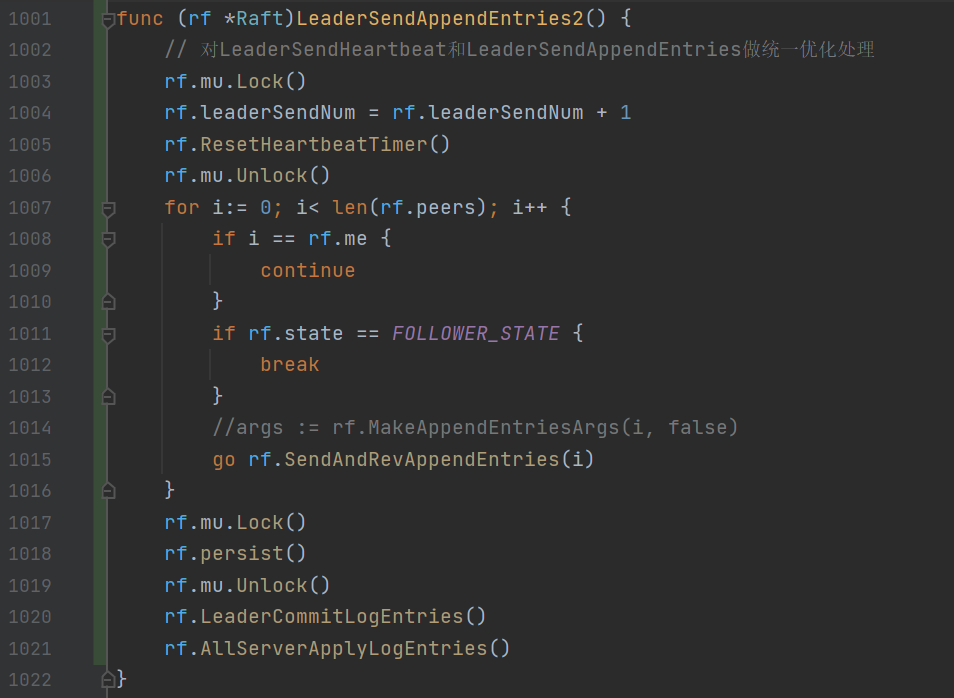
\includegraphics[scale=0.3]{pic3.png}
  \caption{LeaderSendAppendEntries实现}
 %% \Description{This is an example of list in distributed systems.}
\end{figure}

接收者的AppendEntries较为冗杂,为了更好地协调leader和follower,我在AppendEntriesArgs结构体中多加了一个LeaderSendNum变量,因为网络中出现乱序是非常正常的,follower很有可能收到一个过期的包,那么这个包对follower来说帮助并不大,甚至对其做过多处理的话会导致log和leader处的nextIndex等数据回退,加剧了工作量,所以通过这个LeaderSendNum变量来限定收到的RPC一定是来自leader的最新的RPC。

在AppendEntriesReply中加入了Contain、NextTestIndex、Newest变量,Contain取代了论文中Success的工作,代表该follower是否含有prevLogIndex、preLogTerm的日志项,原来的Success代表是否接受了这个RPC。Newest类比于args中的LeaderSendNum,若LeaderSendNum是当前看到已知最大的,那么Newest就为true,代表follower告诉leader这是我收到的最新的RPC,那么leader就认为处理这个reply是有必要的,否则Newest为false代表这个args是陈旧的,那么没有处理的必要。NextTestIndex代表follower告诉leader自己想收到从NextTestIndex开始的日志项。当Contain为true,那么代表PrevLogIndex之前的都已经存入,现在想要更新的日志项且从NextTestIndex开始;当Contain为false,代表PrevLogIndex处的日志项不匹配,需要回退到NextTestIndex开始的位置发送新的日志项。基于NextTestIndex这个变量,我们就能够实现一次性回退多个的思想,提升了效率。

\subsection{step5.一些琐碎的工作}

LeaderCommitLogEntries指leader通过matchIndex数组更新自己的commitIndex,该函数会在每次leader发送AppendEntries后被调用一次进行更新。这里我进行了比较小的优化,按照论文的意思,对当前commitIndex+1开始,若有一个多数派的matchIndex不小于该数,那么这个Index的日志项是可被提交的,这里我使用一个数组来统计每个Index下match的server数量,这样可以节约很多比较产生的时间。这里需要注意的是leader更新commitIndex后会把自己最新的commitIndex在AppendEntries RPC中携带发给follower,follower根据该项更新自己的commitIndex,但是需要注意不能超过自己日志长度,即在args.LeaderCommit和len(rf.log)取一个较小值。

AllServerApplyLogEntries指当commitIndex大于lastApplied时,可以把从lastApplied+1到commitIndex的日志项apply到自动机中,在这里代表传入ApplyMsg类型的信道中。为了使得lastApplied尽量和commitIndex同步,除了在AppendEntries的发送方和接收方函数尾部添加该函数外,在Loop()函数中,当select选择default时也自动执行AllServerApplyLogEntries。

persist和readPersist用于数据持久化,使得部分重要的数据在服务器crash之后的恢复过程中能够从stable storage中读取这部分重要数据,从而更快地恢复成集群中的一员而不使得leader发来的日志项过多导致网络负担较大。这里我选择持久化的数据有currentTerm、voteFor、electionTimeOut、log。以及在各个函数中当上述变量发生更改时会在后续中调用persist更新数据。

基于上面在AppendEntries两个结构体中多加的变量用于提升日志复制效率,在Raft节点中加入了一个新的Boolean型变量consistent,仅供同步阶段的follower使用,当leader发来的RPC中follower含有对应PrevLogIndex、PrevLogTerm处的日志项时,reply中的Contain设为true,并导致自己的变量consistent也变为true,代表自己已经不需要回退了,这样下次再收到RPC时根据自己的consistent为true,可以直接开始加入日志项而不用考虑回退nextIndex的问题。但是这会带来另一个问题,就是当leader crash后,新的leader发来RPC这时候和新的leader的日志并不一定是从nextIndex开始匹配的,所以当发现voteFor不等于收到的RPC中的LeaderId或RPC中的Term比自己的currentTerm大时,就重置consistent为false。

\section{完成情况}
Part1、2、3必做和选做部分均已完成,但是Persist2、Figure8Unreliable的通过率大概在一半左右,UnreliableChurn也大概10次会有一次fail,其他用例没有发现错误。疑似原因是这样的:

\begin{itemize}
    \item 实验有一定延迟,Persist2中错误的那些情况经打印数据发现基本是leader还没来得及将最新的那一个日志项发送给所有server,部分server就被关闭,导致最后报出failed to reach agreement的错误提示。
    \item 怀疑AppendEntries后来由于优化性能加入了一些新定义的参数后,有可能也把bug带进来了,还需要继续优化。
\end{itemize}
实验演示如图3,这是我编写了一个简单脚本循环测试程序20次的截图。(有时测试中会看到Persist2和Figure8Unreliable失败的情况)


  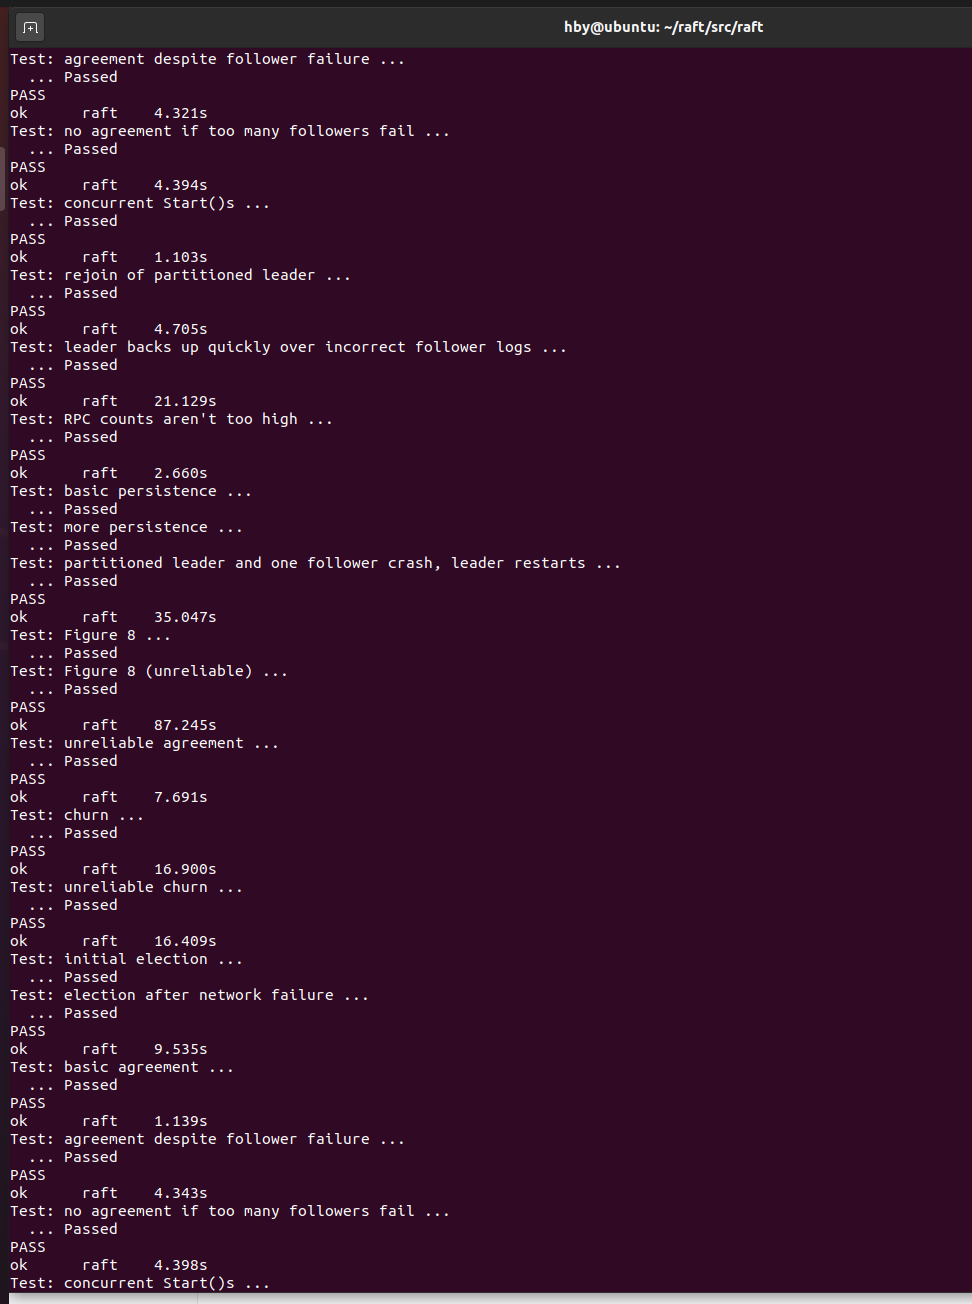
\includegraphics[scale=0.4]{pic2.png}


\section{总结}

\subsection{一路上遇到的困难}
这次大实验一路上遇到了很多bug。

最开始,卡在了TestReElection,检查到错误原因是server2 断连后,server0与server1循环选举,并判断到对方的term更大而转为follower,从此往复。后来找到原因是在FolCanStartElection中,reply.Term > rf.currentTerm写成了rf.me。

后来,卡在TestBasicAgree,检查到错误原因是刚开始各自选主发送heartbeat等正常,后来变成server1与server3进入candidate且死循环,从此往复。很明显,server0、2、4在这里没有crash或延迟,测试后发现server2成为leader后发heartbeat+AppendEntries+heartbeat后,在第二个heartbeat处卡死,最终锁定问题:leader在发AppendEntries后sleep一段时间内下一个heartbeat触发leader执行heartbeat,此时还没经历AppendEntries的LeaderCommitLogEntries,所以发出去的prevLogIndex、prevLogIndex是过期的,后来使nextIndex=matchIndex=0。

再后来,依然卡在TestBasicAgree,错误原因:commitIndex与matchIndex问题,follower端的commitIndex和LastApplied迟迟不动。后来找到原因,Index时从1开始的,所有与日志项有关的包括index、commitIndex等,现在开始给所有需要偏移1的变量进行偏移,在这一步上我修改了很多处很细节的地方,花了不少时间。

再后来,卡在Persist2,有不少报错原因是panic:send on closed channel,这让我想到是在RequestVote处理中,由于某一部分测试设置的传输延迟较大,导致我关闭了信道后还有部分reply朝信道中发送导致panic,于是我使用互斥信号量和一个Boolean来约束当信道关闭后,无法再有reply朝信道中传输。

\subsection{后续工作}

由于我的工作和Raft有关系,所以能够完善自己写的这份代码是非常有必要的,首先我需要优化AppendEntries函数,在不降低性能的情况下将里面的逻辑写的更清晰,其次我需要优化Loop()函数,因为for循环内的最外层循环使用角色来判断进入哪一个分支无疑是更符合逻辑的,而且也能够省去部分定时器的开销。

\subsection{致谢}

这次大实验让我对共识协议有了更深的认识,尽管我原来的工作就是共识协议,但是由于刚进组,对共识协议如Paxos、Raft、ZAB等都是停留在纸面上和规约证明上,这次从code的角度让我对Raft有了更深的认识,让我发现我以前看论文的时候以为自己读懂了,但其实有很多细节的地方也并没有弄得很清楚。最后,感谢老师和助教这一学期的工作!

%\begin{algorithm}[h]
 % \caption{Loop}
 % \label{Loop}
%  \begin{algorithmic}[1]
 %   \Require
 %     Enter .....;
 %   \Ensure
 %     Outpur......
 %   \While{(true)}
%		\State select
%%		\State \qquad case<-rf.electionTimer.C
%		\State \qquad \qquad rf.ResetElectionTimer()
%		\State var newLeader := false
%		   \If {rf.state = FOLLOWER\_STATE}
%				\State rf.FolCanStartElection()
	%		\ElsIf {rf.state = CANDIDATE\_STATE \&\& newLeader = true}
	%			\State rf.FolCanStartElection()
	%		\ElsIf {rf.state = LEADER\_STATE}
%				\State rf.CandidateBecomeLeader()
%				\State go rf.LeaderSendHeartbeat()
	%	 \EndIf
%		\State end select
%	 \EndWhile
 %   \State state2......
 %   \State state3......
 %   \While{(a$>$b)}
 
  %      \State  state4......
  %      \If { c$<$d}
  %          \State state5......
  %      \Else
  %          \State state6......
  %      \EndIf
 %       \State state7......
 %   \EndWhile
 % \end{algorithmic}
%\end{algorithm}

%\begin{figure}[h]
%  \centering
%  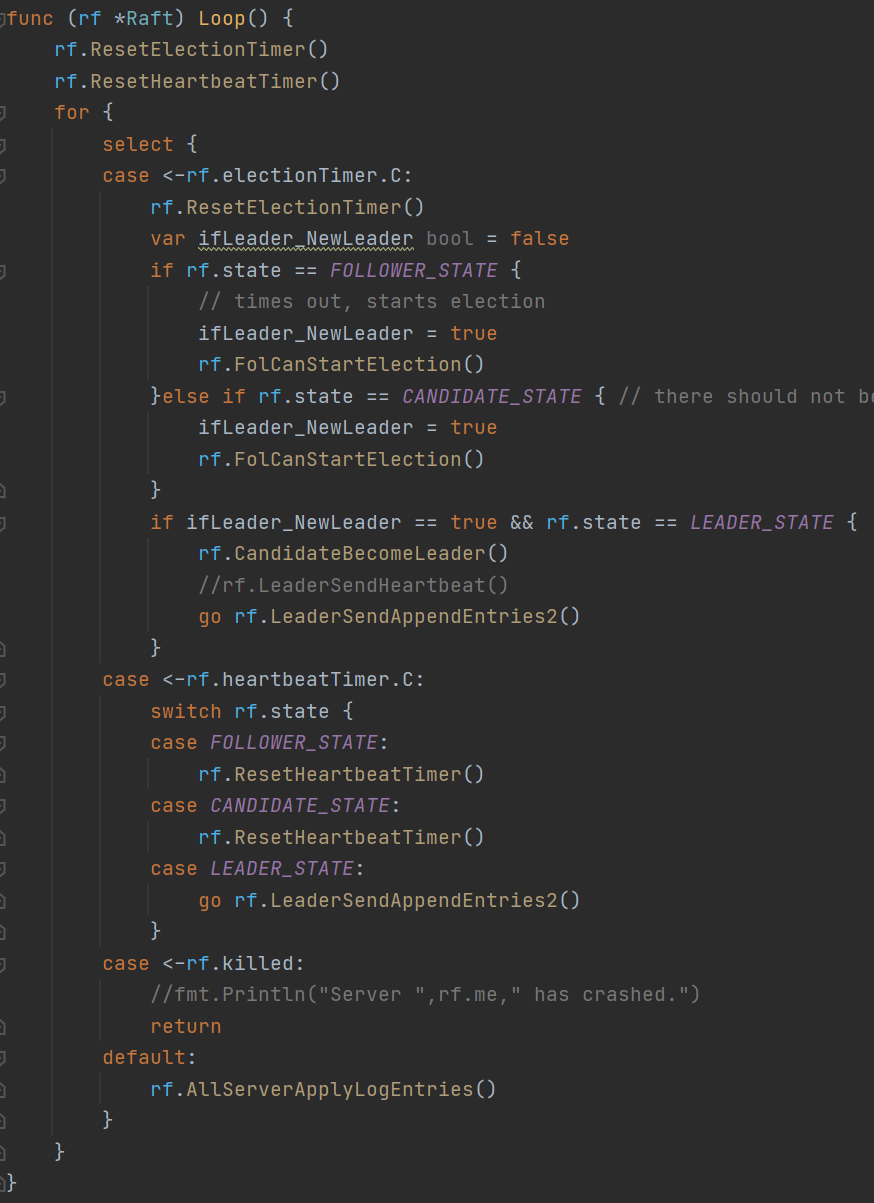
\includegraphics[scale=0.6]{pic1.png}
%  \caption{图灵机中除转移函数外参数的定义}
 %% \Description{This is an example of list in distributed systems.}
%\end{figure}





\end{document}